\documentclass{standalone}
\usepackage{xcolor}
\usepackage{tikz}
\usetikzlibrary{positioning, shapes.multipart, calc, graphs, graphs.standard}
\begin{document}
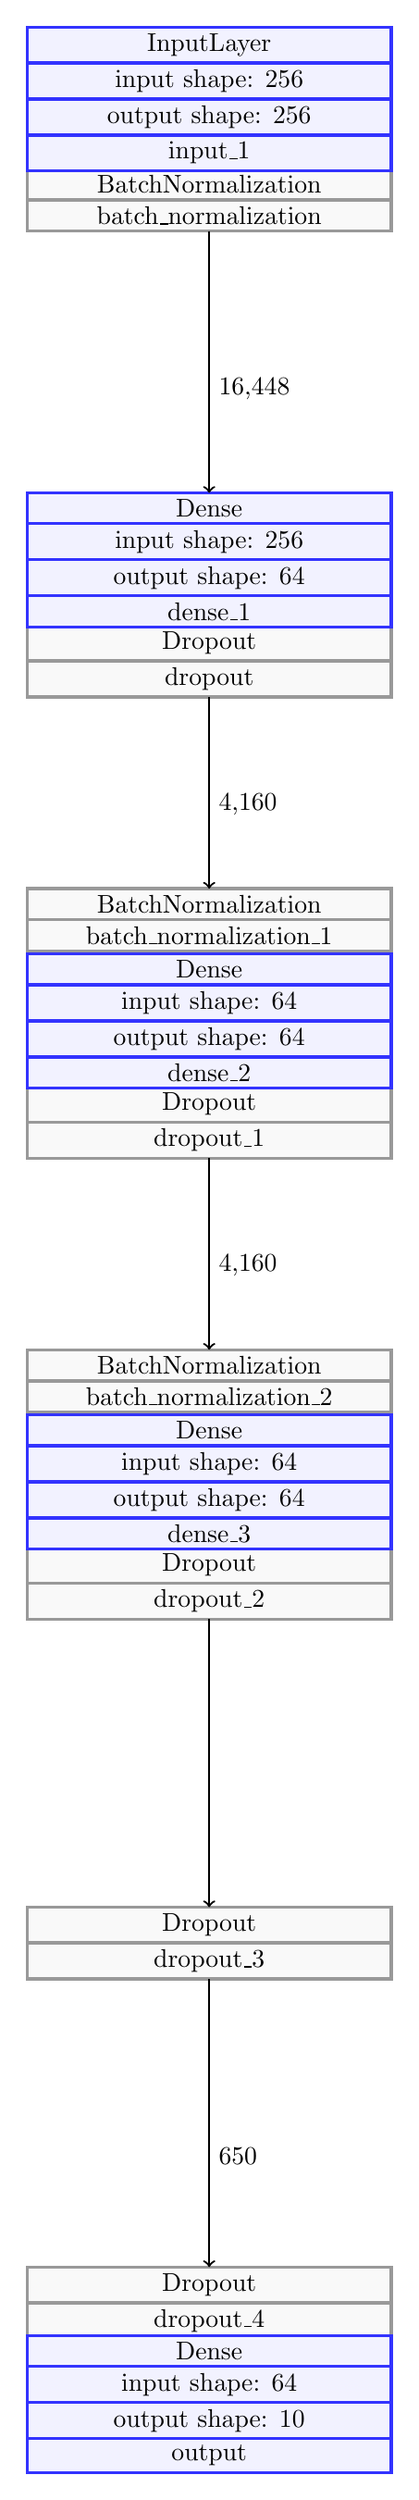
\begin{tikzpicture}[x=30pt, y=30pt]
% style: major_grid
\tikzstyle{major_grid}=[black,step=20pt]
% style: minor_grid
\tikzstyle{minor_grid}=[very thin,step=10pt]
% style: defaultEdge
\tikzstyle{defaultEdge}=[thick,out=-90,in=90,out distance=2cm,in distance=2cm]
% style: defaultLabel
\tikzstyle{defaultLabel}=[auto,pos=0.65]
% style: OperationLayer_style
\tikzstyle{OperationLayer_style}=[rectangle split,rectangle split ignore empty parts,very thick,rectangle split parts=5,draw=violet!80,fill=violet!5,minimum width=5cm,outer sep=0cm,inner sep=2pt]
% style: UtilityLayer_style
\tikzstyle{UtilityLayer_style}=[rectangle split,rectangle split ignore empty parts,very thick,rectangle split parts=5,draw=gray!80,fill=gray!5,minimum width=5cm,outer sep=0cm,inner sep=2pt]
% style: TrainableLayer_style
\tikzstyle{TrainableLayer_style}=[rectangle split,rectangle split ignore empty parts,very thick,rectangle split parts=5,draw=blue!80,fill=blue!5,minimum width=5cm,outer sep=0cm,inner sep=2pt]

% node group: input_1_group
% node: batch_normalization
\node[UtilityLayer_style] (batch_normalization) at (0, 28.683333333333334)
    {
    \nodepart{one}{BatchNormalization}
    \nodepart{two}{batch\_normalization}};
% node: input_1
\node[TrainableLayer_style] (input_1) at (0, 30.0)
    {
    \nodepart{one}{InputLayer}
    \nodepart{two}{input shape: 256}
    \nodepart{three}{output shape: 256}
    \nodepart{four}{input\_1}};
% end of node group: input_1_group

% node group: dense_1_group
% node: dropout
\node[UtilityLayer_style] (dropout) at (0, 22.683333333333334)
    {
    \nodepart{one}{Dropout}
    \nodepart{two}{dropout}};
% node: dense_1
\node[TrainableLayer_style] (dense_1) at (0, 24.0)
    {
    \nodepart{one}{Dense}
    \nodepart{two}{input shape: 256}
    \nodepart{three}{output shape: 64}
    \nodepart{four}{dense\_1}};
% end of node group: dense_1_group

% node group: dense_2_group
% node: batch_normalization_1
\node[UtilityLayer_style] (batch_normalization_1) at (0, 19.316666666666666)
    {
    \nodepart{one}{BatchNormalization}
    \nodepart{two}{batch\_normalization\_1}};
% node: dropout_1
\node[UtilityLayer_style] (dropout_1) at (0, 16.683333333333334)
    {
    \nodepart{one}{Dropout}
    \nodepart{two}{dropout\_1}};
% node: dense_2
\node[TrainableLayer_style] (dense_2) at (0, 18.0)
    {
    \nodepart{one}{Dense}
    \nodepart{two}{input shape: 64}
    \nodepart{three}{output shape: 64}
    \nodepart{four}{dense\_2}};
% end of node group: dense_2_group

% node group: dense_3_group
% node: batch_normalization_2
\node[UtilityLayer_style] (batch_normalization_2) at (0, 13.316666666666666)
    {
    \nodepart{one}{BatchNormalization}
    \nodepart{two}{batch\_normalization\_2}};
% node: dropout_2
\node[UtilityLayer_style] (dropout_2) at (0, 10.683333333333334)
    {
    \nodepart{one}{Dropout}
    \nodepart{two}{dropout\_2}};
% node: dense_3
\node[TrainableLayer_style] (dense_3) at (0, 12.0)
    {
    \nodepart{one}{Dense}
    \nodepart{two}{input shape: 64}
    \nodepart{three}{output shape: 64}
    \nodepart{four}{dense\_3}};
% end of node group: dense_3_group

% node group: dropout_3_group
% node: dropout_3
\node[UtilityLayer_style] (dropout_3) at (0, 6.0)
    {
    \nodepart{one}{Dropout}
    \nodepart{two}{dropout\_3}};
% end of node group: dropout_3_group

% node group: output_group
% node: dropout_4
\node[UtilityLayer_style] (dropout_4) at (0, 1.3166666666666667)
    {
    \nodepart{one}{Dropout}
    \nodepart{two}{dropout\_4}};
% node: output
\node[TrainableLayer_style] (output) at (0, 0.0)
    {
    \nodepart{one}{Dense}
    \nodepart{two}{input shape: 64}
    \nodepart{three}{output shape: 10}
    \nodepart{four}{output}};
% end of node group: output_group

% edge from batch_normalization to dense_1
\draw[->, defaultEdge] (batch_normalization) to node [defaultLabel] {16,448} (dense_1);

% edge from dropout to batch_normalization_1
\draw[->, defaultEdge] (dropout) to node [defaultLabel] {4,160} (batch_normalization_1);

% edge from dropout_1 to batch_normalization_2
\draw[->, defaultEdge] (dropout_1) to node [defaultLabel] {4,160} (batch_normalization_2);

% edge from dropout_2 to dropout_3
\draw[->, defaultEdge] (dropout_2) to node [defaultLabel] {} (dropout_3);

% edge from dropout_3 to dropout_4
\draw[->, defaultEdge] (dropout_3) to node [defaultLabel] {650} (dropout_4);

\end{tikzpicture}\end{document}